% !Mode:: "TeX:UTF-8" 

\BiChapter{基于聚类的克隆代码演化特征分析方法}
{An Analysis for Code Clone Evolutionary Characteristic Based on Clustering Method}

\BiSection{引言}
{Introduction}

为节约开发时间、提高开发效率,复用软件中的既有代码已成为了一种常见的软件开发手段。但是,复用既有代码会向软件系统中引入大量的克隆代码,即彼此相似的代码片段。克隆代码在软件系统中不是静止不变的,会随着软件系统的更新而进行演化,研究人员将克隆代码的这一现象称之为克隆演化。在克隆代码及其演化过程中,必然存在着一些隐含的信息,本文将之称为克隆代码演化特征。克隆演化特征不仅可以帮助软件开发人员理解系统中存在的克隆代码,还可以向软件开发人员提供一些如何维护克隆代码的建议。但遗憾的是,当前研究中对克隆演化特征的研究较为罕见,因此如何分析并获得克隆代码演化特征是一个值得研究的问题。

为了帮助程序开发人员获得克隆代码演化特征,本问结合机器学习中的聚类分析方法,在提取克隆代码相应度量值的基础上揭示了克隆演化特征,可以帮助理解和维护克隆代码。为了描述克隆代码演化过程,本文构建了软件系统的克隆家系,并定义了几种克隆模式用于描述克隆代码演化过程。然后,本文从三个不同的角度描述了克隆代码及其演化过程,即提取不同度量值分别表示克隆片段、克隆组和克隆家系,并在此基础上使用聚类分析的方法挖掘克隆代码的演化特征。在两个开源系统上进行了实验分析,实验结果表明:在演化过程中大部分的克隆代码是较为稳定的,但也存在一定数量的发生变化的克隆代码;在发生变化的克隆代码中,发生一致性变化的克隆代码要多于不一致变化的克隆代码。
%因此, 本文建议开发人员应该更加关注寿命较长的克隆代码,同时当克隆代码发生变化时应考虑是否需要将变化传播到同组的克隆代码中从而满足一致性。

\BiSection{克隆代码演化特征}
{The Code Clone Evolutionary Characteristics}

\BiSubsection{克隆家系定义}
{Code Clone Genealogy}

软件中存在大量的克隆代码,为了收集系统中存在的克隆代码,在过去的20年中,研究人员提出了许多种克隆代码检测方法,并开发了大量的克隆检测工具,例如NiCad\cite{roy2008nicad}、CCFinder\cite{kamiya2002ccfinder}等。有兴趣的读者可以参考本文绪论部分。克隆检测工具从系统源代码中检测克隆代码,并向程序开发人员报告检测结果。克隆检测结果往往以克隆片段和克隆组的形式进行组织:

\begin{itemize}
\item 
\textbf{克隆片段}:克隆片段(\emph{Clone Fragment, CF})是一段代码片段,包括若干行连续的代码。克隆片段与其它的代码片段彼此相似,称之为克隆代码。
\item
\textbf{克隆组}:克隆组 (\emph{Clone Group, CG})是克隆片段的集合,包含几个彼此相似的克隆代码。克隆组揭示了同一克隆组内的克隆片段之间的克隆关系。
\end{itemize}

如绪论所述,克隆代码在系统中不是静止不变的,其也会随着软件系统的演化同时进行演化。克隆演化过程分析最早是2001年由Antoniol等人提出的,他们使用时间序列描述克隆代码的演化模型\cite{antoniol2001modeling},但并未引起人们的重视。2005年,Kim提出了克隆家系模型用于描述克隆代码的演化过程,被认为是迄今为止最好的演化模型,并已成为克隆演化分析的事实标准\cite{kim2005empirical}。Kim等人于同时定义了几种克隆演化模式描述克隆代码在演化过程中的变化情况\cite{kim2005empirical}。克隆家系及其演化模式可以描述如下:
\begin{itemize}
\item 
\textbf{克隆家系}:克隆家系 (\emph{Clone Genealogy, CGE})是一个有向无环图,描述了一个克隆组(CG)随系统进行演化的情况。图中的节点表示某一个系统版本($V_i$)中的该克隆组($CG_i$),图中的边表示该克隆组在相邻的两个版本中的演化关系。
\item
\textbf{克隆演化模式}:克隆演化模式 (\emph{Clone Evolution Pattern, CEP})是某一克隆组在演化中的相邻两个版本的演化模式,用于描述该克隆组的变化情况,具有不同的演化模式。
\end{itemize}

为了更为形象的描述克隆家系,本文给出一个克隆家系的示意图,如图~\ref{gena1}所示。从图中可以看出,克隆家系(CGE)是克隆组(CG)演化的有向无环图,图的节点表示克隆组,图中边表示克隆组的演化关系和演化模式。图中给出一个克隆组在五个版本$(V_i-V_{i+4})$中的演化过程。

\begin{figure}[htbp]
\centering
\includegraphics [width=0.6 \textwidth ]{Fig2-2.pdf}
\bicaption [gena1]{}{克隆家系示意图}{Fig.$\!$}
{An Example for Clone Genealogy}
\vspace{-1em}
\end{figure}

如图中所示,在克隆组的演化过程中,两个版本间的克隆代码可能会发生变化,从而会导致克隆组也发生变化。研究人员使用克隆演化模式描述克隆组的变化情况,本文给出如下7种不同的演化模式描述,如下所示:
%%本课题组同样使用克隆演化模式描述克隆组的变化情况,给出如下7种不同的演化模式描述\icte{}\cite{},如下所示:
\begin{itemize}
\item 
{Static Pattern}:静态模式,表示克隆组未发生任何变化,即组内的克隆片段数量和内容均未发生变化。
\item 
{Same Pattern}:相同模式,表示克隆组内克隆片段数量无变化,但克隆片段本身可能发生变化。
\item 
{Add Pattern}:增加模式,表示克隆组内的克隆片段数量增加。
\item 
{Subtract Pattern}:减少模式,表示克隆组内的克隆片段数量减少。
\item 
{Consistent Change Pattern}: 一致性变化模式,表示克隆组内的克隆片段发生了一致地变化,并且仍然存在同一克隆组内。
\item 
{Inconsistent Change Pattern}:不一致性变化模式,表示克隆组内的克隆片段发生了不一致地变化,并且仍然存在同一克隆组内。
\item 
{Split Pattern}:分裂模式,表示克隆组内克隆片段发生剧烈变化导致克隆组分裂成为两个不同的克隆组。
\end{itemize}

回归到图~\ref{gena1}中,我们可以看出在五个版本内该克隆组的演化模式分布情况。从版本\emph{$V_i$}到{\em $V_i+1$},克隆组新增加了两个克隆片段,因此与之其关联的克隆模式是\emph{Add}。从\emph{$V_i+1$}到{\em $V_i+2$}中,克隆组首先分裂为两组,因此其演化模式为\emph{Split},同时下方的克隆组发生了一致地变化,演化模式为\emph{Consistent Change}。从版本\emph{$V_i+2$}到{\em $V_i+3$}中,演化模式一个是\emph{Subtract},另一个是\emph{Inconsistent Change}。 从版本\emph{$V_i+2$}到\emph{$V_i+ 3$},克隆模式分别是\emph{Add}和\emph{Subtract}。

\BiSubsection{克隆演化特征}
{Clone Evolutionary Characteristics}

克隆家系的提出引发了人们对于克隆代码演化以及演化模式的研究热潮,进而也导致了大量的分析克隆演化特征的研究。克隆演化特征指的是克隆代码在演化过程中表现出来的演化特征或演化模式以及对软件质量的影响。克隆演化特征不仅可以帮助软件开发人员理解系统中存在的克隆代码,还可以向软件开发人员提供一些如何维护克隆代码的建议。

%克隆寿命是指克隆代码在系统中的存在时间,即生存期。Kim研究发现克隆代码要比非克隆代码更加稳定,同时寿命也更长\cite{kim2005empirical};进一步对长寿命的克隆代码进行研究后,发现对克隆代码的修改会使得克隆代码的寿命变短\cite{cai2011empirical}。Krinke通过对比克隆和非克隆代码,也发现克隆代码比非克隆代码的寿命更长\cite{krinke2011cloned}。通过对精确克隆和近似克隆的演化分析,发现其在演化过程中所表现出来的共同特点是:尽管克隆代码比率会随着时间而逐渐降低,但克隆代码的存在时间往往都会超过一年\cite{bazrafshan2012evolution}。因此,克隆代码会长时间的存在于系统中,在其生存期间克隆代码往往会发生变化,其变化规律与具体的软件系统相关\cite{gode2009evolution}。

%相对于克隆寿命而言,克隆稳定性关注的是在克隆代码的生存期内是发生变化的问题。被研究者普遍认可的观点是寿命较长的克隆代码是稳定的\cite{krinke2008cloned}\cite{gode2011clone}\cite{harder2013cloned},不会对系统造成不利的影响,也不会增加系统的维护成本。但是在克隆代码是否比非克隆代码更稳定这个问题上还存在一定的分歧。例如Gode研究发现大部分克隆是稳定的,不会发生变化\cite{gode2011frequency}。而Rahman的研究却发现克隆代码比非克隆代码更容易发生变化,是不稳定的\cite{rahman2014change}。Mondal给出了更为细致的分析结果,即Type 1、Type 2克隆是不稳定的,Type 3克隆是稳定的;并且发现克隆代码比非克隆代码的变化更分散,Type 3克隆比Type 1和Type 2克隆的变化更分散\cite{mondal2012comparative}\cite{mondal2012dispersion}。由此可见,在克隆代码的稳定性特征方面尚未达成共识,仍需要进一步研究。

%克隆代码的变化包括一致性变化和不一致性变化。开发人员遗忘一致性变化将会引发相关的软件缺陷,如标识符重命名不一致性缺陷等,因此一致性变化也是克隆演化分析研究中需要关注的特征。 Gode的研究发现发生一致性变化的克隆代码占克隆代码的比例很小\cite{gode2011frequency}。Krinke的研究进一步发现发生一致性变化和不一致性变化的克隆代码比例大约各占一半,并且大部分发生不一致性变化的克隆代码在后续的演化过程中不会继续发生变化\cite{Krinke2007}。Mondal等人的研究发现发生一致性变化的克隆代码可能会导致延迟传播现象。延迟传播是指某一个克隆片段的变化没有立即传播到其所在的克隆组中,而在间隔一定数量的版本后传播,继续发生一致性变化。研究表明延迟传播在Type 3的克隆中出现的更为频繁,软件开发人员应该重点关注Type 3克隆代码的变化,以避免引入克隆代码相关的软件缺陷\cite{mondal2016comparative}。

究竟哪些演化特征能真实准确地反映克隆代码的规律?这是克隆演化特征分析的难点问题。目前对克隆演化特征的分析主要集中在克隆寿命、克隆稳定性与一致性变化上。(本文表~\ref{characteristic}~列出了目前对克隆演化特征的研究情况。)上述三个特征并不是相互独立的,克隆寿命会受到稳定性和克隆变化的影响,同时克隆稳定性与克隆变化之间存在对立关系,但是目前的研究中并没有揭示这些关系。更为重要的是,对克隆演化特征的研究大多属于实证研究,往往会较多地依赖于研究者的主观态度以及具体被用于实验分析的软件系统,这就导致了不同的研究可能得出不同的结论。例如对克隆稳定性的研究就出现了截然相反的观点。因此,理解克隆代码的存在及其演化过程,并分析克隆代码对软件开发和维护过程产生什么样的影响是十分必要的。克隆演化特征可以实质地帮助克隆维护和管理过程,还可以从演化的角度提供一些全新的建议和理解。

为分析克隆代码及其演化过程,本文基于机器学习方法提出了一种探索和分析克隆演化特征的方法。首先通过映射相邻版本的克隆代码构建系统的克隆家系,并识别克隆组的演化模式用于描述克隆组的演化及其变化情况。然后分别从三个不同的角度表示克隆代码及其演化过程:克隆片段、克隆组和克隆家系,并提取相应的度量值表示不同的克隆实体的感兴趣和有价值的克隆信息。最后,我们使用WEKA( “Waikato Environment for Knowledge Analysis” \cite{hall2009weka})中实现的X-means\cite{pelleg2000x}方法聚类所有的克隆代码。在两个软件系统上进行了实证研究,实证研究结果表明了本文方法可以分析克隆代码的演化特征,可以帮助程序人员理解和维护克隆代码。具体来讲,克隆代在其演化过程中是较为稳定的,在其演化的初始阶段不容易发生变化。程序开打人员因此应该需要更多的关注那些在系统中存在了一定时间的克隆代码(寿命较长的克隆代码)。同时,当克隆代码发生变化的时候,我们也建议尽可能的考虑一致性变化。

%本文的创新点如下:
%\begin{itemize}
%\item 
%本文提出了一个框架分析克隆代码的演化特征,可以帮助程序维护人员维护和管理克隆代码。
%\item 
%本文从三个不同的角度视为将克隆代码一种数据进行分析:克隆片段、克隆组和克隆家系,并提取了相应的度量值表示克隆代码。
%\item 
%本文在两个开源系统上进行了实证研究并获得了相关的克隆演化特征,可以帮助理解和维护克隆代码。
%\end{itemize}

\BiSection{基于聚类的克隆代码演化特征分析框架}
{The Framework for Clone Characteristic Analysis based on Clustering}

本文的基于聚类的克隆代码演化特征分析框架如图~\ref{framework2}所示。该方法可将其划分为三个阶段,分别是预处理阶段、度量提取阶段和演化特征分析阶段。 在预处理阶段,将通过映射连续软件版本之间的克隆代码片以及克隆组来构建相应的克隆家系。并在此基础上识别克隆组的演化模式表示克隆组的演化情况。 在度量提取阶段,从三个不同的角度分别提取不同的度量值表示克隆代码和演化过程,即克隆片段、克隆组和克隆家系。这些所提取的度量值捕获了克隆代码及其进化的相关信息。 最后,在演化特征分析阶段,我们使用机器学习方法中的聚类方法来挖掘克隆代码的克隆演化特征。

\begin{figure}[htbp]
\centering
\includegraphics [width=0.8 \textwidth ]{Fig2-1.pdf}
\bicaption [framework2]{}{基于聚类的克隆演化特征提取方法框架}{Fig.$\!$}
{The Framework of Clone Characteristic Analysis}\vspace{-1em}
\end{figure}

值得注意的是,本文方法将克隆代码及其演化过程当做一种数据,然后借助机器学习领域中的聚类分析方法挖掘隐含的信息。在使用聚类分析的时候,由于克隆代码是具体的代码片段,无法直接对其聚类分析。因此,提取相应的度量值用于表示克隆代码及其演化过程。所采用的聚类分析方法为\emph{X-Means}聚类,其原因在于对于克隆代码具有较少的领域知识,难以确定聚类的数量。而采用人为划分的方式给出聚类的数量,则可能会引入不客观因素,对演化特征分析带来不确定因素。因此,本文采用\emph{X-Means}聚类方法,不需要人为的指定聚类数量,\emph{X-Means}方法会自动地给出最佳的聚类数量。

于此同时,为从不同的角度揭示克隆演化特征,本文将从三个角度分析克隆代码的演化特征,即克隆片段、克隆组和克隆家系。克隆片段是微观角度,从克隆代码自身角度出发,将从克隆代码片段本身是否被修改的角度分析克隆代码的变化性。克隆组是区域角度,从一个克隆组角度分析, 将揭示克隆组的在随着软件演化时的特征。克隆家系是宏观角度,从一个系统中所有的克隆代码(即全部克隆家系)的演化过程。


\BiSection{预处理阶段}
{ Pre-processing}

在这个阶段,我们的目标是根据克隆检测工具所检测的连续版本软件中的克隆代码构建克隆系谱。我们首先获得连续版本的开源软件,主要来源于网站和版本控制系统,并用NiCad检测每个软件版本中的所有克隆代码。NiCad会根据克隆代码的相似性将所有的克隆代码划分为克隆组。之后,我们使用CRD描述克隆代码,并通过关联相邻的克隆片段和克隆组来构建克隆系谱。

\BiSubsection{克隆代码检测与表示}
{Clone Detection and Representation}

%{\em 使用NiCad进行克隆检测和使用CRD(克隆区域描述符)进行克隆表示}。

为了检测系统中的克隆代码,本文使用\emph{NiCad}\cite{roy2008nicad}检测系统中的克隆代码。NiCad是基于Text的克隆检测工具,可以有效地检测系统中的Type-1、Type-2和Type-3的克隆代码。首先,从网站下载系统的每一个版本的源代码。然后,我们使用NiCad的默认配置检测每个软件版本的所有克隆代码。
%NiCad可以从两个不同粒度检测克隆代码:函数克隆和块克隆。因为{\em 块级别}更通用(函数克隆也是是块克隆代码),我们使用{\em 块级别}的默认配置来检测每个软件版本的所有克隆代码。
所检测的克隆代码保存于XML文件中,并使用\emph{``Filename + Line No''}标记克隆克隆代码,同时彼此相似的克隆代码保存在同一克隆组内。

为了构建克隆家系,我们使用修改后的克隆区域描述符(Clone Region Description, CRD)来描述克隆代码。CRD由Duala-Ekoko等人提出,可以抽象的描述克隆代码,具体使用文件名、方法名并结合句法、结构和词法信息等\cite{duala2010clone}。为了使用CRD帮助映射两个相邻版本中的克隆代码和克隆组进行版本间的映射,本文新增\emph{ LocationOverlapping}和\emph{ TextSimilarity}来描述克隆代码的相对位置\cite{}。{\em LocationOverlapping}可以帮助找到源代码中的克隆片段\cite{kim2005empirical},并计算版本$ i $和版本$ i + 1 $中克隆片段位置之间的重叠分数。{\em TextSimilarity}可以用于比较克隆片段的相似性,这里使用NiCad中的计算方法。它计算两个克隆片段的常用代码行的百分比。
%%添加详细的算法描述。

\BiSubsection{克隆家系构建与克隆模式识别}
{Building Clone Genealogy and Identifying Representation}

%%{\em映射克隆组以及构建克隆家系}。
为构建系统中的克隆家系,我们将两个连续版本之间所有的克隆片段和克隆组进行映射,映射算法称为基于CRD的克隆组映射算法\cite{}。给定两个相邻的软件版本\emph{$V_i$}和\emph{$V_ {i + 1}$},我们将\emph{$V_i$}中的每个克隆片段与下一版本\emph{$ V_{i+1}$}中的每个克隆片段进行比较,寻找与之映射的克隆片段。根据克隆片段的映射结果,同时映射相邻版本中的所有的克隆组。 
%%算法的细节在我们前面的工作[25]中描述。
克隆组映射后,可以使用演化模式描述克隆组在两个版本之间的变化,即\emph{``Clone Pattern''}。假设存在于两个相邻版本中的一个克隆组,使用\emph{srcCG}表示前一版本中的克隆组,\emph{destCG}表示后一版本中的克隆组,从\emph{srcCG}到\emph{destCG}的变化由克隆模式描述。接下来通过遍历所有版本之间的映射的克隆组可以构建系统中的克隆家系。


\BiSection{提取阶段}
{Extracting Clone Metrics}

正如在机器学习中通常所做的那样,我们将使用度量值表示克隆代码,并将之称为\emph{克隆代码度量}。如前文所述,本文将从三个角度提取度量值表示克隆代码,即克隆片段、克隆组和克隆家系。

\BiSubsection{克隆片段度量}
{Clone Metrics for Clone Fragment}

克隆片段度量给出了克隆代码本身的一些特征。在克隆片段的生命期间,克隆片段可能被程序人员开发人员修改(特别是在软件维护期间)。因此,克隆片段在演化过程中会发生变化,并且可能发生不止一次的变化。因此,本文将克隆代码的变化次数和从上一版本演化到此版本时是否发生了变化视为克隆代码的度量。 因此,在某一软件版本$V_ i $中的克隆代码片段表示如下:
\begin{itemize}
\item
克隆寿命(Clone Life):截止到当前版本$V_ i $,克隆片段$CF$所经历的所有的版本数量称之为克隆寿命。
%\item {Clone Life}: number of versions which the clone fragment exists in software so far (until version i).
\item
是否发生变化(Ischanged):软件版本$V_ i $中的克隆片段$CF$是否在上一版本到这一版本演化时发生了变化,若发生变化则取值为$1$,否则取值为$0$。
%\item {Ischanged}:	equals 1 if the Clone fragment in version i is changed from the last version (version i-1); 0 otherwise.
\item
变化次数(Change Times):截止到当前版本$V_ i $,克隆片段$CF$在其演化过程中所发生的变化次数。
%\item {Change Times}:	number of times the clone fragment changed so far (up till version i) in the evolution.  
\end{itemize}

\BiSubsection{克隆组度量}
{Clone Metrics for Clone Group}

克隆组提供了克隆代码的一些区域性特征。由于本文所使用的克隆演化模式均是针对克隆组的演化情况,因此本文也需要从克隆组的角度分析克隆代码的演化情况。
%这里的克隆组是指在同一版本中的克隆代码所组织成的克隆组。
对于某一个克隆组,本文最先提取的度量是克隆寿命。克隆寿命不但揭示了其在系统中存在的时间长短,也与克隆演化模式息息相关。在克隆组进行演化的过程中,克隆模式更是从演化的角度揭示了克隆组的变化情况。因此,我们将版本$V_i $ 中克隆组的寿命和克隆模式提取为度量值,如下所示:
\begin{itemize}
\item
克隆寿命(Group Life):截止到当前版本$V_ i $,克隆组$CG$所经历的所有的版本数量称之为克隆寿命。
%\item {Group Life}: number of versions which clone group exists in software till version $i$.
\item
静态(Static):克隆组$CG$从上一版本演化到$V_ i $时,其演化模式为静态模式。
%\item {Static}:	all clone fragments in group are static from last version.
\item
相同(Same):克隆组$CG$从上一版本演化到$V_ i $时,其演化模式为相同模式。
%\item {Same}:	clone group undergoes a ``same'' pattern change from  last version.
\item
增加(Add):克隆组$CG$从上一版本演化到$V_ i $时,其演化模式为增加模式。
%\item {Add}: clone group undergoes an ``add'' pattern change from last version.
\item
减少(Subtract):克隆组$CG$从上一版本演化到$V_ i $时,其演化模式为减少模式。
%\item {Subtract}: clone group undergoes a ``subtract'' pattern change from last version.
\item
一致性变化(Consistent Change):克隆组$CG$从上一版本演化到$V_ i $时,其演化模式为一致性变化模式。
%\item {Consistent Change}: clone group undergoes a ``consistent change'' pattern from last version.
\item
不一致变化(Inconsistent Change):克隆组$CG$从上一版本演化到$V_ i $时,其演化模式为不一致变化模式。
%\item {Inconsistent Change}: clone group undergoes an ``inconsistent change'' pattern from last version.
\item
分裂(Split):克隆组$CG$从上一版本演化到$V_ i $时,其演化模式为分裂模式。
%\item {Split}: clone group undergoes a ``split'' pattern change from last version.
\end{itemize}

\BiSubsection{克隆家系度量}
{Clone Metrics for Clone Genealogy}

克隆家系可以提供一个软件中克隆代码演化的全局视角,从而可以帮助我们捕获所有版本中的整个克隆代码演化的特征。如前文所述,一个克隆组在所有的版本中的演化过程即是一个克隆家系,因此一个软件系统中有很多个克隆家系。对于每一个克隆家系,本文提取了\emph{克隆寿命}和\emph{克隆模式数量}度量来表示克隆家系。\emph{克隆寿命系}的重要指标,它描述了克隆家系在系统中生存的时间。克隆家系描述了这个克隆组在整个生命中如何演化(克隆模式),从而通过这些信息可以告诉我们关于克隆家系变化的历史。因此,本文提取了克隆家系在其整个生命中经历的\emph{克隆寿命}和\emph{克隆模式数量},如下所示:

\begin{itemize}
\item
克隆家系寿命(Genealogy  Life):克隆家系整个演化过程中所经历的软件版本的数量。
%\item Genealogy  Life: number of versions which clone genealogy exists in software.
\item
静态模式数量(Static Number):克隆家系在整个演化过程中所经历的静态模式的数量。
%\item Static Number: number of ``static'' pattern which all clone groups belonging to this genealogy have experienced in its life.
\item
相同模式数量(Same Number):克隆家系在整个演化过程中所经历的相同模式的数量。
%\item Same Number: number of ``same'' pattern which all clone groups belonging to this genealogy have experienced in its life.
\item
增加模式数量(Add Number):克隆家系在整个演化过程中所经历的增加模式的数量。
%\item Add Number: number of ``add'' pattern which all clone groups belonging to this genealogy have experienced  in its life.
\item
减少模式数量(Subtract Number):克隆家系在整个演化过程中所经历的减少模式的数量。
%\item Subtract Number: number of ``subtract'' pattern which all clone groups belonging to this genealogy have experienced in its life.
\item
一致性变化模式数量(Consistent Number):克隆家系在整个演化过程中所经历的一致性变化模式的数量。
%\item Consistent Number: number of ``consistent pattern'' which all clone groups belonging to this genealogy have experienced in its life.
\item
不一致变化模式数量(Inconsistent Number):克隆家系在整个演化过程中所经历的不一致变化模式的数量。
%\item Inconsistent Number: number of ``inconsistent pattern'' which all clone groups belonging to this clone genealogy have experienced in its life.
\item
分裂模式数量(Split Number):克隆家系在整个演化过程中所经历的分裂模式的数量。
%\item Split Number: number of ``split'' pattern which all clone groups belonging to this genealogy have experienced in its life.
\end{itemize}

\BiSection{克隆演化特征挖掘}
{Clone Evolutionary Characteristics Mining}

为了从克隆代码及其演化过程中挖掘演化特征,我们将使用WEKA\cite{}中提供的聚类方法来分析克隆代码,从克隆片段、克隆组和克隆家系三个不同的角度进行分析。本文将上述每一个克隆片段、克隆组和克隆家系统一称之为克隆实体。本文将这个挖掘任务分成两个子任务:第一,我们对获得的所有克隆实体进行统计分析,并且根据统计分析结果获取克隆代码的演化特征。第二,我们使用WEKA对克隆实体进行聚类分析。在这个子任务中,主要目标是分析在软件演化过程中克隆代码的寿命以及变化情况,即确定克隆变化在克隆演化中所发生的时间以及变化。为此,我们在WEKA中使用工具来对包含时间元素的克隆实体进行聚类。在这个子任务中,使用WEKA完成此任务也涉及两个部分:首先,我们为每一个克隆实体成一个“克隆演化向量”,其中包含每个克隆代码的所有度量(包括时间度量)。然后,我们使用WEKA聚类这些向量,并从聚类获得的结果中分析并获取克隆演化特征。

\BiSubsection{克隆演化向量}
{Clone Evolutionary Vector}

 \emph{生成克隆向量}。 对于每个克隆片段、克隆组和克隆家系,其特征向量是一个$m$维向量:{$V$ ={($v_1$,$v_2$,$...$,$v_m$)}},其中$v_i$表示前面章节中提到的特定度量。为所有克隆生成向量后,获得所有克隆的聚类向量空间$X$,其可以由{$X$={($x_1$,$x_2$,$...$,$x_n$)}}表示,其中$n$是克隆实体的数量。我们从三个角度考虑克隆:克隆片段,克隆组和克隆家系。以克隆组为例,一个克隆组产生一个8维向量{$V$ =($v_1$,$v_2$,$...$,$v_8$)},其中$v_i$(对于所有$i$ , $i \leq $ 8)是此克隆组所提取的度量值。
  
 \emph{ 使用WEKA聚类克隆特征向量}。WEKA是一种用于数据挖掘的机器学习工具。我们将克隆作为数据并产生相应的实体而不是克隆代码,然后使用WEKA分析所有载体(所有克隆)以获得克隆特征。 WEKA中实现了许多方法来分析数据,例如聚类,分类,关联规则等。我们对矢量空间X上的克隆片段,克隆组和克隆家系使用{\em X-means Clustering}算法。 {\ em X-means clustering}是{\ em k-means}的变体;后者旨在将$ n $向量分割为先前指定的$ k $数量的簇,使得每个向量属于其平均值最接近该向量的簇。假如使用{\ em K-means},我们需要确定聚类之前的数量。然而,对于克隆分析的情况,难以确定所需的簇的数目。因此,我们使用{\ em X-means clustering}。

\BiSubsection{X-means聚类方法}
{X-means Clustering Method}

X-means聚类是一种高效的算法,可以自动的搜索聚类位置的空间和优化贝叶斯信息准则度量所需的聚类数量\cite{}[26],它可以自动确定集群的数量。给定一组向量(克隆)$X$ = {($x_1$,$x_2$,$...$,$x_n$)},其中每个$x_i$是$d$维实向量)。X-means聚类旨在将这些$n$向量划分为$k$ clusters $C$ = {($C_1$,$C_2$,$...$,$C_k$)},以便最小化群内平方和(WCSS)(聚类中每个点的距离函数与K中心的距离函数的和),集群中每个点的距离函数与其集群中心的总和)。我们只指定$ K $的范围值。 {\em X-means clustering}可以有效地从范围中搜索最好的$K$。它从给定的$K$范围的最低值开始,并继续增加此值,直到范围的上限。在此过程中,X-means聚类使用模型选择标准计算每个$K$的分数。它选择$K$的最高分数输出。对于每个$K$,x-means聚类使用迭代细化技术。首先,它将每个向量分配给其平均值产生集群内最小平方和(WCSS)的集群。第二,它计算新的均值为新聚类中的向量的质心。当分配不再改变时,算法收敛。它使用后验概率用贝叶斯信息准则对这$j$进行评分。

\BiSection{实验结果与分析}
{The Results and Discussion}

在本节中,我们将给出我们的案例研究。首先,我们简要描述了所使用的开源软件系统,并描述了从三个不同的克隆代码视角探索克隆演化特征的实验步骤。我们选择两个开源软件作为我们的实验系统:分别为{\em ArgoUML}和{\em jEdit}。它们都是使用Java语言开发的软件,并且它们都经历了超过10个版本的演化。{\em ArgoUML}是一个领先的开源UML建模工具,包括对所有标准UML 1.4图的支持。{\em jEdit}是另一个开源项目,是程序员开发所使用的编辑器,其特点是具有易于使用的接口,类似于许多流行的文本编辑器。\\

表~\ref{statisticsofcluster}描述了这两个实验系统的基本信息情况。具体来说,我们分别考虑$ 14 $和$ 22 $版本。对于每个软件,我们列出此实验的第一个版本(开始)和最后版本(结束)。列“克隆片段”列出从每个软件收集的克隆片段的数量(包括所有版本)。类似地,“克隆组”和“克隆家系”分别是收集的克隆组和克隆家系的数量。
\begin{table}[htbp]
\bicaption [statisticsofcluster]{}{两个开源软件实验系统信息}{Table$\!$}{The Two Open Sources Software for Experiments}
\vspace{0.5em}\centering \wuhao
\begin{tabular}{ccccccc}
\toprule [1.5pt ]
\multirow{2}{*}{Projects}&\multirow{2}{*}{Versions}&Start&End&Clone&Clone&Clone\\ 
&&Version&Version&Fragment&Group&Genealogy\\
\midrule[1pt]
ArgoUML&14&0.20.0&0.34.0&25422&7012&1036\\ 
jEdit&22&3.0.0&5.0.0&6636&2256	&237\\ 
\bottomrule [1.5pt]
\end{tabular}
\end{table}

为了探索克隆代码演化特征,我们将克隆代码分为三个不同的视角:克隆片段、克隆组和克隆家系。 首先,我们对克隆片段进行实验。 在这里,我们探讨和调查克隆片段从一个版本到另一个版本的变化情况,以及克隆片段的历史变化情况和存在系统中的时间。 其次,克隆组在软件进化过程中有一些克隆模式。 在这里,我们有兴趣确定克隆模式的类型(例如一致的变化,不一致的变化等),它们发生(或不发生)频繁(或不频繁)。最后,克隆家系实验,提供了软件的全局视图。

在每个实验中,我们使用两种方法分析克隆:第一种是使用统计方法分析克隆,第二种使用X-means聚类方法深入分析克隆。

\BiSection{实验结果和分析}{Analysis \& Results}
\BiSubsection{克隆片段实验}{Clone Fragment Experiment}

克隆片段是指软件中存在的真实的代码片段。 在其生命周期内(作为克隆),克隆片段可能会被开发人员修改,特别是在软件维护期间。为帮助分析克隆片段的变化,我们考虑克隆片段的三个度量(相对于检测到它们的软件版本):{\em clone life,ischanged and change time}。 这些将帮助我们了解克隆如何在其演化过程中的变化情况。

\begin{table}[htbp]
\bicaption[cfstaargouml]{}{ArgoUML中克隆片段的变化统计信息}{Table$\!$}{Clone Fragment  Change Statistic of ArgoUML}
\vspace{0.5em}\centering\wuhao
\begin{tabular}{ccccc}
\toprule[1.5pt]
 & \multicolumn{4}{c}{Change Times}\\
\midrule[1pt]
Change Times&0&1&2&3\\ 
Number&24327&982&109&4\\ 
Total&24327&\multicolumn{3}{c}{1095} \\
\bottomrule[1.5pt]
\end{tabular}
\end{table}

\begin{table}[htbp]
\bicaption[cfstajedit]{}{jEdit中克隆片段的变化统计信息}{Table$\!$}{Clone Fragment  Change Statistic of jEdit}
\vspace{0.5em}\centering\wuhao
\begin{tabular}{ccccccccc}
\toprule[1.5pt]
 & \multicolumn{8}{c}{Change Times}\\
\midrule[1pt]
Change Times &0&1&2&3&4&5&6&7\\ 
Number&5885&533&135&47&14&10&11&1\\ 
Total&5885&\multicolumn{7}{c}{751}   \\ 
\bottomrule[1.5pt]
\end{tabular}
\end{table}

在表~\ref{cfstaargouml}和表~\ref{cfstajedit}中,我们对克隆片段的变化进行了统计分析。从表中可以看到,大多数克隆片段在它们的演化过程中不会发生变化(在{\em ArgoUML}中为$24327$,在{\em jEdit}中为$5885$)。同时, 只有一小部分克隆片段在演化中发生了变化(在{\em ArgoUML}为$1095$,{\em jEdit}为$751$)。 还有极少数的克隆片段其生命周期中改变了不止一次。 这里,我们可以得出结论:{\em 克隆片段在其生命中非常稳定(大多数克隆片段从不改变);对于发生变化的,它们不会非常频繁地变化。}

\begin{table}[htbp]
\bicaption[cfcluargouml]{}{ArgoUML中克隆片段的聚类结果}{Table$\!$}{Clone Fragment Clustering Results of ArgoUML}
\vspace{0.5em}\centering\wuhao
\begin{tabular}{ccccccccccc}
\toprule[1.5pt]
\multirow{3}{*}{Cluster}&{Number}&\multicolumn{3}{c}{Clone Life}&\multicolumn{3}{c}{Ischanged}&\multicolumn{3}{c}{Change Times} \\
&(Percentage)&\multirow{2}{*}{Mean}& Standard &\multirow{2}{*}{Median}&\multirow{2}{*}{Mean}&Standard &\multirow{2}{*}{Median}&\multirow{2}{*}{Mean}&Standard &\multirow{2}{*}{Median}\\
&&&  Deviation&&& Deviation&&& Deviation&\\ 
\midrule[1pt]
Cluster 0&899(4\%)&7.2069&2.2993&7&0.09232&0.28965&0&1.13014&0.34963&1\\ 
Cluster 1&3082(12\%)&7.76314&1.52307&8&0&0&0	&0&0&0\\ 
Cluster 2&3006(12\%)&3.833&0.8707&4&0.05822&0.23419	&0	&0.0652&0.24692&0\\ 
Cluster 3&18435(73\%)&1.09401&0.29184	&1	&0	&0	&0	&0	&0	&0\\ 
\bottomrule[1.5pt]
\end{tabular}
\end{table}

\begin{table}[htbp]
\bicaption[cfclujedit]{}{jEdit中克隆片段的聚类结果}{Table$\!$}{Clone Fragment Clustering Results of jEdit}
\vspace{0.5em}\centering\wuhao
\begin{tabular}{ccccccccccc}
\toprule[1.5pt]
\multirow{3}{*}{Cluster}&{Number}&\multicolumn{3}{c}{Clone Life}&\multicolumn{3}{c}{Ischanged}&\multicolumn{3}{c}{Change Times} \\
&(Percentage)&\multirow{2}{*}{Mean}& Standard &\multirow{2}{*}{Median}&\multirow{2}{*}{Mean}&Standard &\multirow{2}{*}{Median}&\multirow{2}{*}{Mean}&Standard &\multirow{2}{*}{Median}\\
&&&  Deviation&&& Deviation&&& Deviation&\\ 
\midrule[1pt]
Cluster 0&	200(3\%)	&5.325	&2.6899	&5	&1	&0	&1	&1.64	&1.1476	&1\\ 
Cluster 1&	1371(21\%)	&9.07075	&2.88542	&8	&0	&0	&0	&0.50328	&0.91649	&0\\ 
Cluster 2&	1624(15\%)	&4.2266	&1.11192	&4	&0	&0	&0	&0.06466	&0.26059	&0\\ 
Cluster 3&	3441(66\%)	&1.17495	&0.37998	&1	&0	&0	&0	&0	&0	&0\\ 
\bottomrule[1.5pt]
\end{tabular}
\end{table}

在表~\ref{cfcluargouml}和~\ref{cfclujedit}是克隆片段的聚类结果。对于{\em ArgoUML}和{\em jEdit}两个开源软件中,Cluster0是所有克隆片段中数量最小的,该Cluster中的克隆代码从上一个版本演化到此版本时发生了变化,我们将此克隆称为{\em changed clone}。从表中可以看到{\em 在所有的克隆代码中很少发生变化的克隆片段,同时对于发生变化的克隆代码,发生变化的时刻往往是当它们在系统中存在一段时间后}。根据``{\em isChanged}''列,我们可以看到对于{\em  ArgoUML}中的Cluster1和3和{\em  jEdit}中的Cluster1、2和3,所有的克隆片段都没有发生变化。这意味着{\em 大多数克隆片段在其演化的过程中是稳定的}。{\em ArgoUML}和{\em jEdit}中的Cluster3是完全没有发生变化的克隆片段,根据其寿命发现它们在软件中存在的寿命极短 。这表明{\em 刚刚出现在系统中的克隆是“极其”稳定的(它们在短时间内不会发生变化)}。因此,我们应该更多地关注{\em 克隆片段存在几个版本,因为他们更容易发生变化。}

总之,只有少数的克隆代码片段在软件演化过程中会发生变化。 这些变化的克隆所经历的的变化往往通常发生在它们在系统中存在一段时间之后经历变化。

\BiSubsection{克隆组实验}{Clone Group Experiment} 

{\em clone fragment}仅仅可以提供克隆片段本身的演化属性,是一个最小的角度。而通过对{\em clone group}进行分析则提供了一个较大的角度分析克隆代码的演化情况。 %在软件演化的上下文中。每个版本的软件都有很多克隆组。
我们研究克隆组在进化过程中是如何变化的。这些更改按{\ em clone patterns}分类。

\begin{table}[htbp]
\bicaption[cgstaargouml]{}{ArgoUML中克隆组的变化统计信息}{Table$\!$}{Clone Group  Change Statistic of ArgoUML}
\vspace{0.5em}
\centering\wuhao
\begin{tabular}{cccccccc}
\toprule[1.5pt]
Number of&\multirow{2}{*}{Static}&\multirow{2}{*}{Same}&\multirow{2}{*}{Add}&\multirow{2}{*}{Subtract}&Consistent&Inconsistent&\multirow{2}{*}{Split}\\ 
Groups&&&&&Change&Change&\\ 
\midrule[1pt]
Metric is Present	&5114	&5422	&345	&324	&350	&329	&36\\ 
Metric is Absent	&1898	&1590	&6667	&6688	&6662	&6683	&6976\\ 
Percentage	&72.93\%	&77.40\%	&4.92\%	&4.62\%	&5.25\%	&4.69\%	&0.51\%\\ 
\bottomrule[1.5pt]
\end{tabular}
\end{table}

\begin{table}[htbp]
\bicaption[cgstajedit]{}{jEdit中克隆组的变化统计信息}{Table$\!$}{Clone Group  Change Statistic of jEdit}
\vspace{0.5em}\centering\wuhao
\begin{tabular}{cccccccc}
\toprule[1.5pt]
Number of&\multirow{2}{*}{Static}&\multirow{2}{*}{Same}&\multirow{2}{*}{Add}&\multirow{2}{*}{Subtract}&Consistent&Inconsistent&\multirow{2}{*}{Split}\\ 
Groups&&&&&Change&Change&\\ 
\midrule[1pt]
Metric is Present	&1783	&1922	&45	&36	&140	&41	&19\\ 
Metric is Absent	&473	&334	&2211	&2220	&2116	&2215	&2237\\ 
Percentage	&79.3\%	&85.20\%	&1.99\%	&1.60\%	&6.21\%	&1.82\%	&0.84\%\\ 
\bottomrule[1.5pt]
\end{tabular}
\end{table}

如表~\ref{cgstaargouml}和~\ref{cgstajedit}所示,我们计算每个{\em clone pattern}的克隆组数。我们使用“Present”和“Absent”来指示克隆组是否具有克隆模式。我们非正式地将克隆模式“静态”和“同一”称为{\ em稳定克隆模式},其他作为{\em dynamic clone pattern}。对于两个项目,{\em 大多数克隆组(72 \% - 85 \%)有稳定的克隆模式,只有一小部分克隆组$ ^ 1 $ {注: jEdit中的克隆模式非常小。 (2)克隆组可以有多个度量,包括分配给一个组的“Add”和“Subtract”。}(每个小于5 \%)有动态克隆模式它们与模式的关联,例如添加,减去,拆分,一致/不一致的改变)。}此外,我们看到{\ em在ArgoUML和jEdit中仍然有数百个一致/不一致的变化。这应该吸引开发者的注意,因为这种模式 - 特别是不一致的变化 - 可能暗示潜在的克隆缺陷。在{\em  jEdit}中,{\em 一致的变化远不止不一致的变化,而且,在ArgoUML中,一致的变化也比不一致的变化}。似乎{\em 对克隆组中的克隆的一致更改经常发生在软件中}。

\begin{table}[htbp]
\bicaption[cgcluargouml]{}{ArgoUML中克隆组的聚类结果}{Table$\!$}{Clone Group Clustering Results of ArgoUML}
\vspace{0.5em}\centering\wuhao
\begin{tabular}{cccccccccc}
\toprule[1.5pt]
 \multirow{2}{*}&\multirow{2}{*}&Group&Static &Same &Add &Subtract &Consistent &	Inconsistent &Split \\ 
&&Life& Number& Number& Number& Number& Number&	 Number& Number\\ 
\midrule[1pt]
Cluster0&Mean&	3.04167	&0.58712	&0.70076	&1	&1	&0	&1	&0.07955\\ \cline{2-10}
264&Standard Deviation	&2.25093	&0.49329	&0.4588	&0	&0	&0	&0	&0.2711\\ \cline{2-10}
(4\%)&Median	&2	&1	&1	&1  &1	&0	&1	&0\\ \hline
Cluster1&Mean	&4.90926	&1	&1	&0	&0	&0	&4.03307E-4	&6.04961E-4\\ \cline{2-10}
4959&Standard Deviation	&3.0984	&0	&0	&0	&0	&0	&0.02008	&0.02459\\ \cline{2-10}
(71\%)&Median	&5	&1	&1	&0	&0	&0	&0	&0\\ \hline
Cluster2&Mean	&3.38795	&0	&0.66988	&0.18554	&0.14458	&0.84337	&0.15181	&0.01928\\ \cline{2-10}
415&Standard Deviation	&2.66601	&0	&0.47082	&0.38921	&0.3521	&0.36389	&0.35927	&0.13766\\ \cline{2-10}
(6\%)&Median	&2	&0	&1	&0	&0	&1	&0	&0\\ \hline
Cluster3&Mean	&0.60844	&0	&0	&0.00291	&0	&0	&0	&0.00291\\ \cline{2-10}
1374&Standard Deviation	&0.52006	&0	&0	&0.0539	&0	&0	&0	&0.0539\\ \cline{2-10}
(20\%)&Median	&1	&0	&0	&0	&0	&0	&0	&0\\
\bottomrule[1.5pt]
\end{tabular}
\end{table}

\begin{table}[htbp]
\bicaption[cgclujedit]{}{jEdit中克隆组的聚类结果}{Table$\!$}{Clone Group Clustering Results of jEdit}
\vspace{0.5em}\centering\wuhao
\begin{tabular}{cccccccccc}
\toprule[1.5pt]
\multicolumn{10}{c}{\bf Table 9.\  Clone Group Clustering Results of jEdit }\\ 
 \multirow{2}{*}&\multirow{2}{*}&Group&Static &Same &Add &Subtract &Consistent &	Inconsistent &Split \\ 
&&Life& Number& Number& Number& Number& Number&	 Number& Number\\ 
\midrule[1pt]
Cluster0&	Mean	&6.88	&0.4	&0.76	&1	&1	&0	&1	&0.2\\ \cline{2-10}
25	&Standard Deviation	&4.43772	&0.5	&0.43589	&0	&0	&0	&0	&0.40825\\ \cline{2-10}
(1\%)	&Median	&7	&0	&1	&1	&1	&0	&1	&0\\ \hline
Cluster1	&Mean	&5.76199	&1	&1	&0	&0	&0	&0	&5.64016E-4\\ \cline{2-10}
1773	&Standard Deviation	&4.05197	&0	&0	&0	&0	&0	&0	&0.02375\\ \cline{2-10}
(79\%)&	Median&	5	&1&	1&	0&	0&	0&	0&	0\\ \hline\
Cluster2	&Mean	&5.36242&	0&	0.87248&	0.12752&	0&	0.9396&	0.02685&	0.0604\\\cline{2-10}
149&	Standard Deviation&	3.77977&	0&	0.33468&	0.33468&	0&	0.23903&	0.16218&	0.23903\\ 
\cline{2-10}
(7\%)&	Median&	4&	0&	1&	0&	0&	1&	0&	0\\ \hline
Cluster3	&Mean	&0.99676&	0&	0	&0.00324	&0.0356	&0	&0.03883	&0.01294\\ \cline{2-10}
309	&Standard Deviation	&1.23924	&0	&0	&0.05689	&0.18559	&0	&0.19351	&0.11322\\ \cline{2-10}
(14\%)&	Median&	1&	0&	0&	0&	0&	0&	0&	0\\ 
\bottomrule[1.5pt]
\end{tabular}
\end{table}

表~\ref{cgcluargouml}和~\ref{cgclujedit}描述了克隆组聚类的结果。这里,集群1具有最大数量的克隆组(71\%在{\em ArgoUML},79\%在{\em jEdit}),这些克隆组相对稳定(具有稳定的克隆模式,没有动态克隆模式),并且具有相对较长的寿命。因此,{\em 大多数克隆组是非常稳定的,其也具有相对较长的寿命(在两个软件中大约5个版本)}。大多数{\em 不一致的更改模式}出现在群集0中,它只占用很小的百分比({\em ArgoUML}中的4\%,在{\em jEdit}中只有1\%)。因此,{\em 不一致的更改在克隆组中不会频繁发生}。同时,{\em  consistent change pattern}仅发生在集群2中,集群2的生命周期相对较长,但比集群0短。集群0和2都是动态克隆组,因为它们都具有动态克隆模式。我们得出结论,{\em 动态克隆模式发生在更长寿的克隆组中,它们的数量非常小}。

如果我们检查群集0 和2中的组的绝对数量,我们看到具有一致变化的克隆组(群集2)的数量大于具有不一致变化的群集(群集0)的数量。这意味着{\em 一致的变化很容易发生比不一致的变化}。因此,我们建议:{\em 开发人员应该考虑在检测到克隆片段已经发生一些变化时执行一致的更改的可能性}。

集群3显示有相当一部分的克隆组具有极短的寿命(刚刚出现在系统中),其没有克隆模式。这意味着{\em 我们不需要考虑在克隆组创建的初始版本克隆组中的更改的影响}。

总之,克隆组在整个进化中通常是非常稳定的。动态克隆模式可能发生在克隆组存在一段时间之后,但只有一小部分。当开发人员更改特定的克隆片段时,建议他们也考虑克隆组上下文中的更改,并确定是否需要在整个组中进行一致的更改。

\BiSubsection{克隆家系实验}{Clone Genalogy Experiment} 

在研究克隆系谱学的特征(其提供全局观点)中,我们首先计算每个克隆系谱在其整个生命中出现的克隆模式的数目,然后使用它们的度量对这些克隆系谱进行聚类。
 
\begin{figure}[htbp]
\centering
\subfigure{\label{cgestas1}}\addtocounter{subfigure}{-2}
\subfigure[ArgoUML分析结果]{\subfigure[ArgoUML]{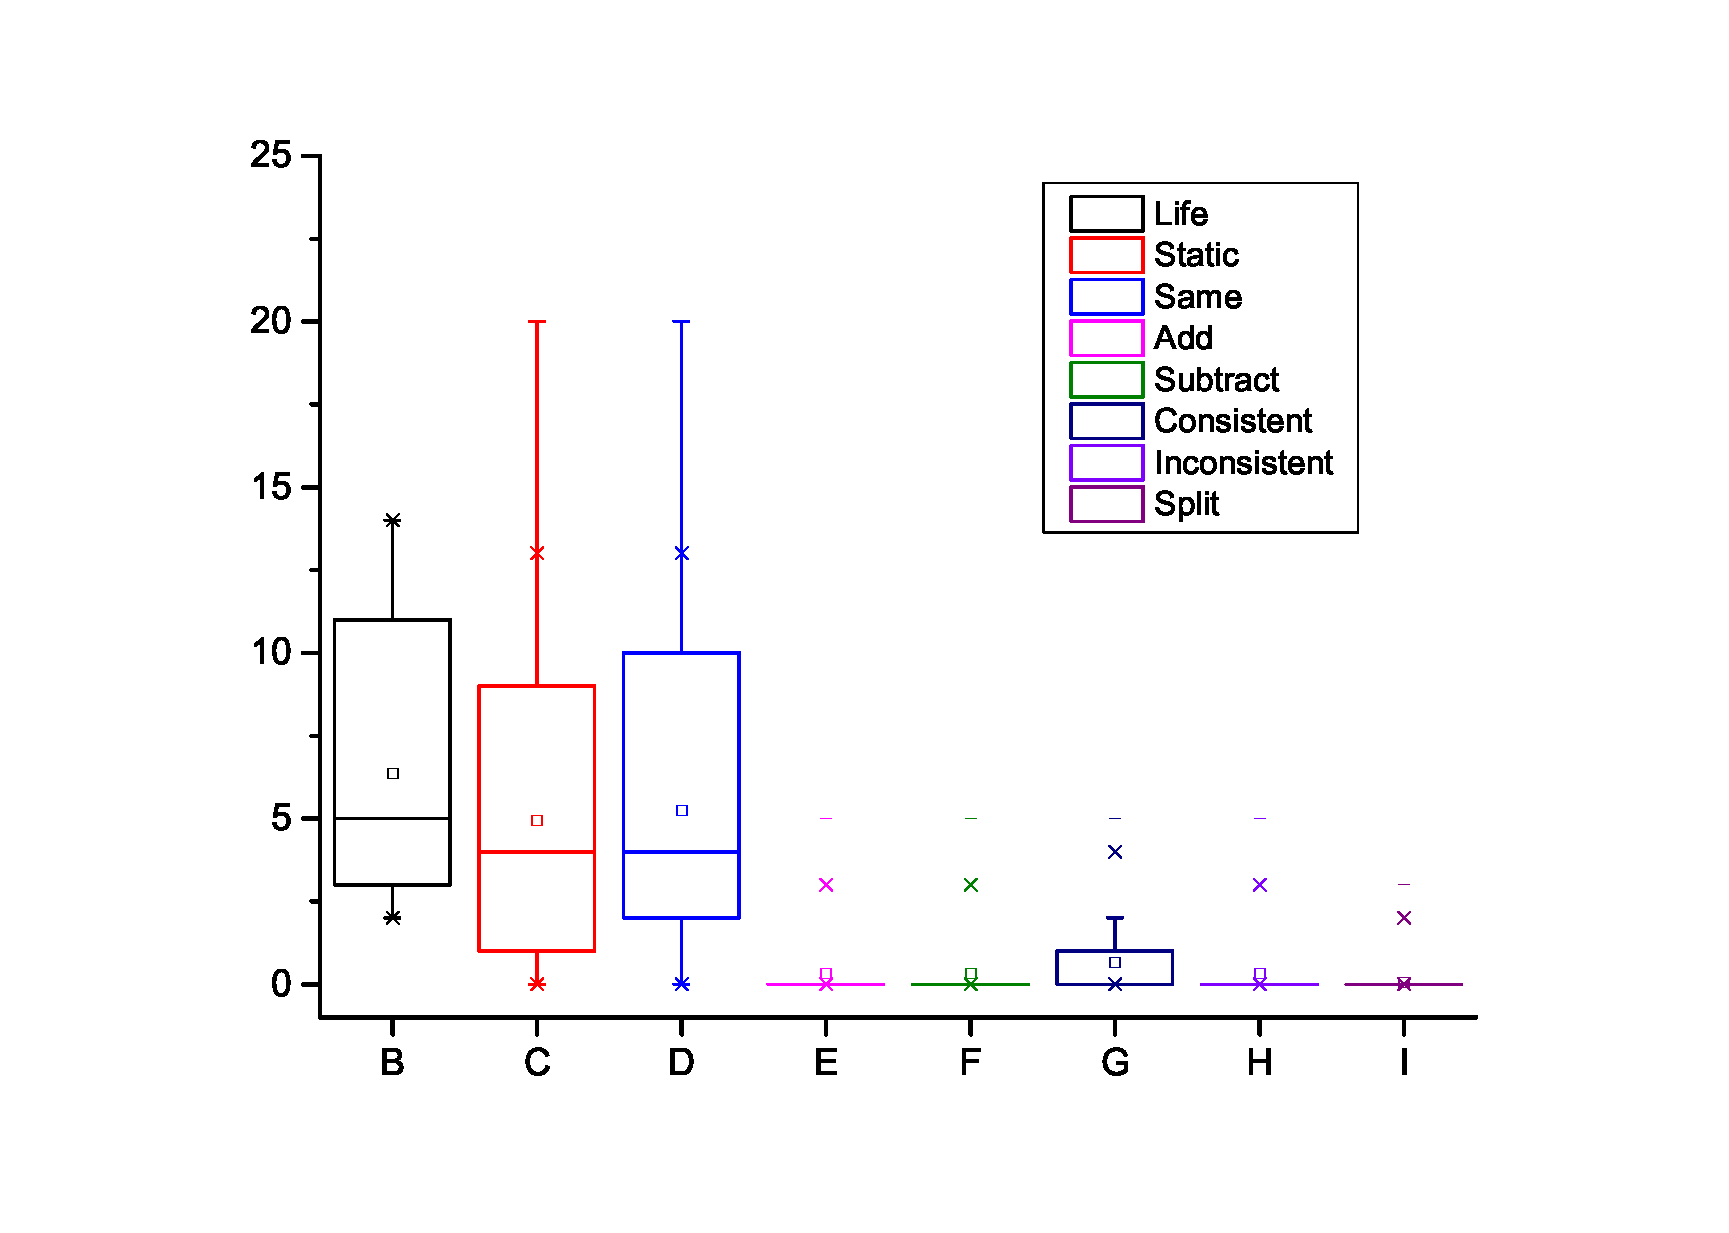
\includegraphics[width=0.4\textwidth]{Fig2-3a.eps}}}
\subfigure{\label{cgestas2}}\addtocounter{subfigure}{-2}
\subfigure[jEdit]{\subfigure[jEdit]{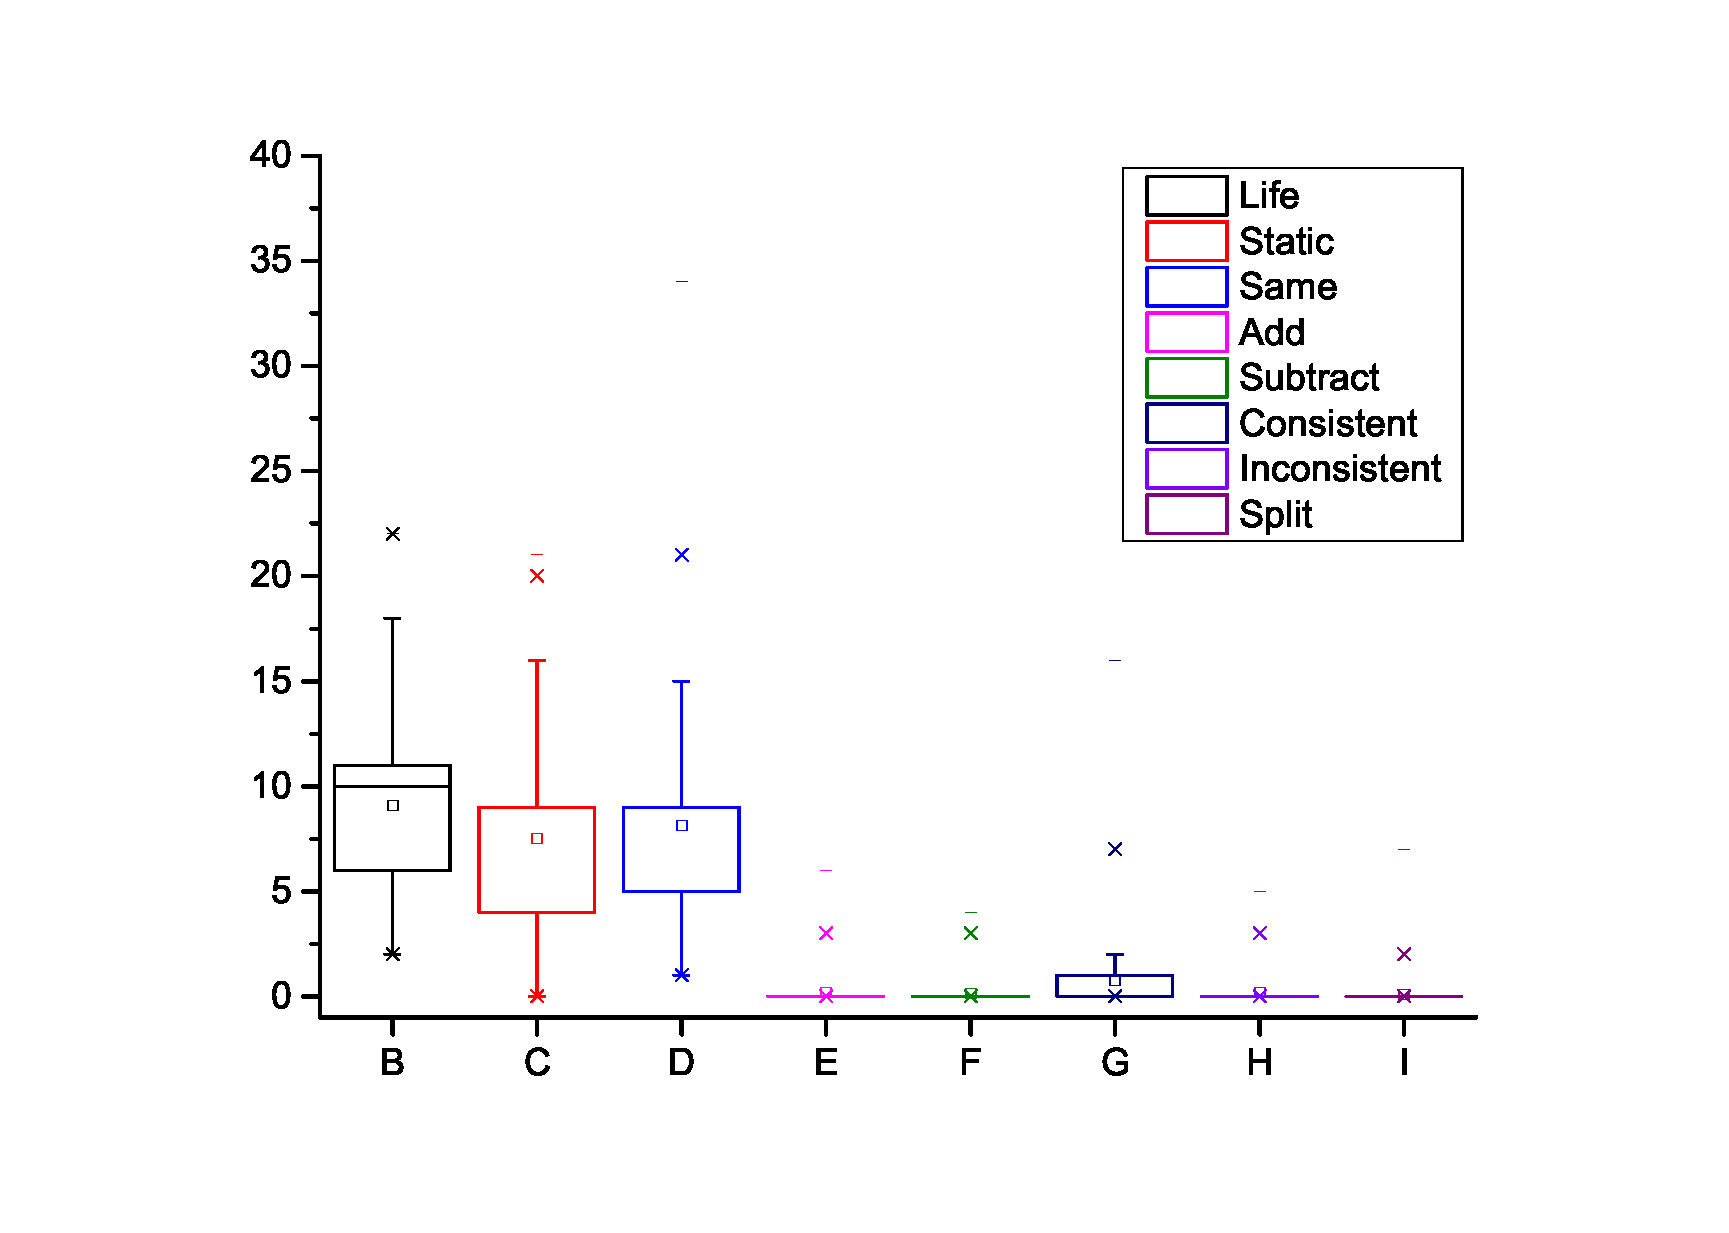
\includegraphics[width=0.4\textwidth]{Fig2-3b.eps}}}
\bicaption[cgestas]{}{克隆家系统计分析结果}{Fig.$\!$}{Clone Genealogy Statistics Results}\vspace{-1em}
\end{figure}

我们首先计算所有克隆谱系中的每个度量(包括谱系生活和克隆模式)的统计。结果绘制在图\ref{},使用“框和须”图。 第一个(最左侧)框显示关于家谱生活的统计。 对于图中的其余框,它们中的每一个代表每个克隆模式的统计。
 
我们可以看到克隆系谱在系统中存在相当长的一段时间(即{\em mean value of life}。是{\em  ArgoUML}在整个14个版本中的5个版本,以及10个版本的{\em jEdit }与整个22版本),并且只有一小部分克隆系谱存在极短(少于3版本)或极长(多于10版本)的生活。我们还看到{\em stable clone pattern}的数量远远高于{\em dynamic clone pattern}的数量。 对于{\em dynamic clone pattern},它们的数量非常少,期望{\em consistent change pattern}。{\em 这意味着克隆系谱在克隆进化的生命期间是非常稳定的。}特别地,“一致的变化”的数量超过“不一致的变化”的数量。 这意味着{\em 值得注意确定克隆更改是否应该传播到同一克隆组中的其他克隆}。
  
\begin{table}[htbp]
\bicaption[cggcluargouml]{}{ArgoUML中克隆家系的聚类结果}{Table$\!$}{Clone Genealogy Clustering Results of ArgoUML}
\vspace{0.5em}\centering\wuhao
\begin{tabular}{ccccccccccc}
\toprule[1.5pt]
 &Death&&Genealogy Life&	Static&	Same&	Add	&Subtract&	Consistent&	Inconsistent&	Split\\ 
\midrule[1pt]
Cluster0&\multirow{3}{*}{5}&Mean	&11.85366	&9.79268	&10.45122	&2.23171&	2.23171&	3.06098&	2.29268&	0.39024\\ \cline{3-11}
82&&Standard Deviation	&1.81979	&2.98861&	3.04758&	1.04585&	1.08068	&0.85125&1.07138&	0.84263\\ \cline{3-11}
(8\%)&&Median	&11&	10&	10&	2&	2&	3&	2	&0\\ \hline
Cluster1&\multirow{3}{*}{39}&Mean	&10.19221	&8.83117	&9.0961	&0.17143	&0.12208	&0.44416	&0.12208	&0.00519\\ \cline{3-11}
385&&Standard Deviation&	1.67998	&1.67552	&1.70282	&0.39754&	0.3278	&0.64761&	0.3278	&0.10193\\ \cline{3-11}
(37\%)&&Median	&11	&9	&10	&0&	0&	0&	0	&0\\ \hline
Cluster2&\multirow{3}{*}{188}&Mean	&3.29412	&1.2549	&2	&0.47059	&0.46078	&1.2598	&0.46078	&0.0098\\ \cline{3-11}
204&&Standard Deviation	&1.22847	&1.35506	&1.32427	&0.63875	&0.63822	&0.43961	&0.63822	&0.14003\\ \cline{3-11}
(20\%)&&Median	&3&	1&	2&	0&	0&	1&	0&	0\\ \hline
Cluster3&\multirow{3}{*}{348}&Mean	&2.79452	&1.79452	&1.79452	&0	&0	&0	&0	&0\\ \cline{3-11}
365&&Standard Deviation	&1.0813	&1.0813	&1.0813	&0	&0	&0	&0	&0\\ \cline{3-11}
(35\%)&&Median	&3	&2	&2	&0	&0	&0&	0&	0\\ \hline
All&\multirow{3}{*}{579}&Mean	&6.35907	&4.93629	&5.23359	&0.33301	&0.31274	&0.65541	&0.31757	&0.03475\\ \cline{3-11}
1036&&Standard Deviation	&4.02533	&4.0219	&4.06154	&0.74995	&0.74514	&0.97405	&0.75663	&0.27231\\ \cline{3-11}
(100\%)&&Median&	5&	4&	4&	0&	0&	0&	0&	0\\ \hline
\bottomrule[1.5pt]
\end{tabular}
\end{table}

\begin{table}[htbp]
\bicaption[cggclujedit]{}{jEdit中克隆家系的聚类结果}{Table$\!$}{Clone Genealogy Clustering Results of jEdit}
\vspace{0.5em}\centering\wuhao
\begin{tabular}{ccccccccccc}
\toprule[1.5pt]
&Death&&Genealogy Life&	Static&	Same&	Add	&Subtract&	Consistent&	Inconsistent&	Split\\
\midrule[1pt]
Cluster0&\multirow{3}{*}{3}&Mean	&19	&15.8	&19.2	&3	&2.3&	6	&2.7&	1.1\\ \cline{3-11}
10&&Standard Deviation	&4.83046	&4.56557&	6.42564	&1.33333&	0.94868&	4.57044&	1.41814	&2.23358\\ \cline{3-11}
(4\%)&&Median	&22&	17&	19&	3&	2	&4.5	&2.5&	0\\ \hline
Cluster1&\multirow{3}{*}{35}&Mean	&10.95205&	9.44521&	9.93836&	0.07534	&0.07534	&0.58904&	0.08219&	0.0411\\ \cline{3-11}
146&&Standard Deviation&2.35572	&2.16566&2.35832	&0.26485	&0.31262&	1.07428&	0.34254&	0.28471\\ \cline{3-11}
(62\%)&&Median&	10&	9&	9	&0&	0	&0	&0&	0\\ \hline
Cluster2&\multirow{3}{*}{24}&Mean	&6.57143&	4.75&	5.60714&	0.07143&	0.07143&	0.85714&	0.07143&	0.07143\\ \cline{3-11}
28&&Standard Deviation	&1.16837&	1.14261	&1.22744	&0.26227&0.26227	&0.97046	&0.26227	&0.37796\\ \cline{3-11}
(12\%)&&Median	&7	&5	&6&	0	&0	&1&	0&	0\\ \hline
Cluster3&\multirow{3}{*}{48}&Mean	&3.33962&	2.13208&	2.30189&	0.03774&	0	&0.20755&	0	&0\\ \cline{3-11}
53&&Standard Deviation&	0.73231	&0.92065	&0.72284&	0.19238&	0&	0.45398	&0	&0\\ \cline{3-11}
(22\%)&&Median	&3&	2&	2	&0&	0&	0	&0&	0\\ \hline
All&\multirow{3}{*}{110}&Mean	&9.07173	&7.52321&	8.1097	&0.18987&	0.1519&	0.76371	&0.173&	0.08017\\ \cline{3-11}
237&&Standard Deviation	&4.36559&	4.07926	&4.56922	&0.6903&	0.55438&	1.70588	&0.66354	&0.55033\\ \cline{3-11}
(100\%)&&Median	&10	&9	&9	&0	&0	&0	&0	&0\\ \hline
\bottomrule[1.5pt]
\end{tabular}
\end{table}

我们使用X-means聚类从{\em life}和{\em 克隆模式}之间的克隆系谱中挖掘更多信息。在表~\ref{}和~\ref{}中,我们定义了一个称为{\em Death}的特殊变量,其报告在达到实验收集的最后版本之前已经结束生命的克隆系谱的数量。通过知道一个家谱有助于{\em Death}中的计数,我们知道我们在克隆系谱实验中获得的数据是“完整的”。家谱不会被我们选择的软件版本过早地终止。因此,这些表中的第二列显示了死亡克隆系谱的编号。

根据聚类结果,所有克隆系谱可以聚类成四个聚类,如表所示。%从图。 3 /表10 \和11,
很明显{\em 在家谱生活和稳定模式之间存在强正相关}。我们非正式地定义一个家谱是{\em stable},如果它具有高百分比的{\em 稳定克隆模式},(由大量的“静态”和“相同”度量表示)。否则,我们说系谱是{\em dynamic},(也就是说,它有一个相对较大的“add”,“subtract”,“ split‘’克隆模式)。从表中,我们可以看到:{\em 大多数克隆系谱是稳定的(簇1,2,3)}。另一方面,动态系谱学少得多(在群集0中,具有长寿命,并且大多数系统中仍然存活)。它告诉我们{\em 动态克隆模式 - 特别是一致和不一致的变化 - 通常发生在更长寿的克隆系谱中。此外,动态系谱的数量很小}。这表明开发人员应该对{\em 动态系谱}采取一些措施,因为不一致的更改可能导致软件缺陷。对于簇3(表10,11中),相应的克隆系谱具有相对较短的寿命,并且它们中的大多数已经死亡。这些克隆系谱非常稳定,因为不存在不一致的模式。 {\em 因此,可以得出结论,短寿命克隆系谱中的克隆比较老的克隆更稳定。它可以给我们一个提示,开发人员可能不需要保持他们的眼睛在新创建(较短的生命)克隆系谱。但是,当他们与软件一起发展时,他们应该注意他们。}

总之,克隆系谱在整个进化中大多是稳定的。较短寿命的家谱特别稳定。 {\em 动态变化模式}通常发生在较长寿命的家谱中,即使外观依然稀少。其中,一致的变化比不一致的变化更频繁。因此,我们建议开发人员应该注意更长寿的克隆系谱,并考虑当一个克隆片段即将发生变化时允许克隆组一致变化的可能性。
 
 \BiSection{讨论和分析}{Discussion}
 
 我们的方法取决于NiCad和克隆映射算法构建克隆系谱。 我们使用NiCad检测克隆,其结果然后用于映射克隆,以便构建克隆系谱。更精细的克隆检测工具和更精确的克隆映射算法可能提高后续阶段的质量。请注意,我们的方法很大程度上取决于克隆度量的可用性。我们使用一组指标来表示克隆片段,克隆组,克隆系谱。虽然这些指标对我们有很好的影响,但我们希望将来扩展指标的收集,因为新的有趣指标可以暗示克隆与其进化之间可能存在的新关系。

在将来,我们还可以对具有更多克隆度量的不同软件进行更多的实验。我们相信,我们提出了一些更有意义的结论,以帮助克隆分析和克隆维护。我们还可以对克隆特征进行一些进一步的工作。我们认为克隆特征应该在系统维护期间的克隆分析中使用。例如,我们可以从软件中识别一些特殊的克隆,并且我们打算将其链接到克隆有害性。

 \BiSection{结论}{Conclusion}
 
在本文中,我们提出了一种通过机器学习方法从克隆及其进化中分析克隆进化特征的方法。具体来说,我们通过考虑克隆实体的生命时间证明了克隆实体的聚类(通过X平均算法)的有用性。我们的论文的贡献包括:(1)我们提出一个框架来分析克隆特征的多版本软件。 (2)我们提取一类相关的克隆度量来表征克隆片段,克隆组和克隆系谱。我们提供了关于克隆进化的三个不同的观点,从而可以从克隆进化的所有方面得出结论,从个体克隆的角度到全球的系谱观点。 (3)我们对两个软件进行了一个案例研究:{\em  ArgoUML}和{\em jEdit}来研究克隆进化特征。我们的案例研究表明克隆通常在其进化过程中非常稳定,并且克隆通常在进化的婴儿期不经历改变。因此,开发人员应该更多地关注在几次进化(也就是更长寿的克隆系谱)后存在于谱系中的(更成熟的)克隆。我们还建议开发人员应考虑在其中一个组成的克隆片段发生变化时,在整个克隆组中进行一致性更改的可能性。

我们相信这些特性可以帮助开发人员更好地理解克隆,还可以提供一些指导来维护和管理软件开发中的克隆。在未来,我们打算通过纳入更多的度量来改进我们对克隆组和克隆基因生态学的分析。关于克隆组和谱系关系的结论可以被看作是克隆进化的特征。这些功能可能有助于克隆管理。